\paragraph{\trBraneStructure。}\label{sub:brane-structures}
现在假设 $M$ 带有一个二次复\trVolume{}形式——在这个维数下，它只是一个无处为零的%
$C^\infty$ 二次\trDifferential{} $\eta_M^2\colon TM\otimes_\CC TM\to\CC$。与之相伴的%
\trSquaredPhase{}映射可以想成实\trProjective{}化\trTangentBundle{}的一个%
\trTrivialization{} $\alpha_M\colon\RP(TM)=Gr(TM)\to S^1$。把它可视化的一条好途径是%
实\trSubbundle{} $\xi_M=\alpha_M^{-1}(1)$，它在\trSurface{}上给出一个无\trOrientation{}%
的\textbf{\trFoliation}（foliation）。在这些词语下，$M$ 中的一个\trLagrange\trBrane{}就是一条\trEmbedding{}的%
闭曲线 $L$，配备有
\begin{itemize}
\item \trPullback{} $\pi^*(TM|L)$ 的一个实\trSubbundle{} $H$，其中
$\pi\colon[0;1]\times L\to L$ 是\trProjection，满足 $H|(\{0\}\times L)=\xi_M|L$ 与%
$H|(\{1\}\times L)=TL$；
\item 一个实\trLineBundle{} $\beta\to L$。
\end{itemize}
$H$ 是 $TM|L$ 的诸\trSubbundle{}之间的一个\trHomotopy，或者更几何地说，是把 $L$ 的%
全部\trTangentSpace{}同时旋转、使之变得平行于 $\xi_M$ 的一种方式。这种\trHomotopy{}%
存在性的\trObstruction{}是 $L$ 相对于 $\xi_M$ 的\textbf{整体\trRotationNumber{}}（winding number，它必须消没这一要求同样%
排除了零\trHomology{}的简单闭曲线）。为了把这段讨论与一般的\trGrading{}概念联系起来，%
注意：若有这样一个 $H$，则存在唯一的函数 $a\colon[0;1]\times L\to\RR$，满足 $a(0,x)=0$%
与 $\exp(2\pi i\,a(r,x))=\alpha_M(H_{r,x})$，而 $\alpha^{\#}(x)=a(1,x)$ 便是 $L$ 的一个%
\trGrading。至于 $\beta$，由\cref{thm:pin1-example} 我们知道，它\trEquivalence{}于一个%
\trPinStructure{}的选取。
设 $\boldsymbol{L}^{\#}$ 是一组处于\trGeneralPosition{}的\trExactLagrangianBrane{}
$L_k^{\#}=(L_k,H_k,\beta_k)$，$1\le k\le m$。我们现在要往先前的构造里加进\trGrading{}%
与符号，得到一个组合式定义的\trDirected{}\trACategory。为此，我们首先对每个交点%
$y\in L_{i_0}\cap L_{i_1}$（$i_0<i_1$）关联一个绝对\trIndex{} $i(y)$ 与一个%
\trOrientation{}空间 $o(y)$。把\trHomotopy{} $H_{i_0}(1-\cdot,y)$ 与 $H_{i_1}(\cdot,y)$%
拼接成 $\RP(TM_y)$ 中一条从 $(TL_{i_0})_y$ 到 $(TL_{i_1})_y$ 的路径。令%
${\lhd}(y)\in\RR\setminus\pi\ZZ$ 为这条路径所转过的总角度，并令
\begin{equation}\label{eq:combinatorial-index-orientation}
i(y)=[{\lhd}(y)/\pi]+1,\qquad
o(y)=\Hom(\beta_{i_0,y},\beta_{i_1,y})\otimes(TL_{i_1})_y^{\otimes\,i(y)}.
\end{equation}
有了这些，我们便照常（\eqref{eq:graded-floer-cochains}）定义\trMorphism{}空间%
$CF^*(L_{i_0}^{\#},L_{i_1}^{\#})$。其次，取一个\trImmersion\trPolygon{}
$\tilde{u}\colon\Delta^{d+1}\to M$，其\trCornerPoint{}位于 $y_0,\ldots,y_d$ 处。用%
\eqref{eq:combinatorial-index-orientation} 作一个简单的计算可知，这种\trPolygon{}的%
存在蕴含等式 $i(y_0)=i(y_1)+\cdots+i(y_d)+2-d$。在诸\trCornerPoint{}处，按%
\cref{fig:immersed-polygon}中箭头所示（注意 $y_0$ 处的约定与 $y_1,\ldots,y_d$ 处%
不同），用 $\Delta^{d+1}$ 的边界\trOrientation{}为 $(TL_{i_d})_{y_0}$ 与%
$(TL_{i_k})_{y_k}$（$k=1,\ldots,d$）赋予\trOrientation。沿 $\Delta^{d+1}$ 诸边的%
\trParallelTransport{}定义了\trIsomorphism{} $\beta_{i_k,y_k}\to\beta_{i_k,y_{k+1}}$%
与 $\beta_{i_d,y_d}\to\beta_{i_d,y_0}$。看一看 \eqref{eq:combinatorial-index-orientation}%
便可发现，这两件初等事实合起来给出一个\trIsomorphism{} $o(y_d)\otimes\cdots\otimes%
o(y_1)\to o(y_0)$，我们把它记作 $\tilde{c}_{\tilde{u}}$。定义
$\tilde{\mu}^d\colon CF^*(L_{i_{d-1}}^{\#},L_{i_d}^{\#})\otimes\cdots\otimes%
CF^*(L_{i_0}^{\#},L_{i_1}^{\#})\to CF^{*+2-d}(L_{i_0}^{\#},L_{i_d}^{\#})$ 为把全部%
\trNormalization{} $|\tilde{c}_{\tilde{u}}|_\KK$ 加起来的结果。一个基于恰有一个凹%
\trCornerPoint{}的\trPolygon{}之分解的初等论证表明，这些映射满足\trAinfty-结合性方程%
\eqref{eq:aoo-associativity}。把按这种方式定义的\trDirected{}\trACategory{}记作%
$\widetilde{\scr{F}}(\boldsymbol{L}^{\#})^{\to}$。
\begin{example}\label{thm:cylinder-two-gon-example}
考虑 $M=S^1\times[-1;1]$，在\cref{fig:cylinder-two-gon}中画成一个两条\trVertical{}边%
被等同起来的方块，其上有曲线 $L_0$、$L_1$。我们使用与由\trHorizontal{}直线组成的%
\trFoliation{} $\xi_M$ 相对应的常值复\trVolume{}形式。对 $L_0$，选取从 $\xi_M|L_0$ 到%
$TL_0$ 的平凡\trHomotopy。另一种情形，$\xi_M|L_1$ 与 $TL_1$ 之间的角度处处小于 $\pi/2$，%
故二者之间有一条唯一的“短”\trHomotopy，我们采用它。最后，取平凡的\trLineBundle{}
$\beta_0$、$\beta_1$。于是 $i(y_0)=0$、$i(y_1)=1$、$o(y_0)=\RR$（\trCanonical{}地，%
因为\trIndex{}是偶数），而 $o(y_1)=(TL_1)_{y_1}$。\cref{fig:immersed-polygon}的约定说，%
在计算二边形 $u$ 对\trBoundaryOperator{}的贡献时，应当用%
\cref{fig:cylinder-two-gon}所示的\trOrientation{}来认同 $o(y_1)\cong\RR$；另一个%
二边形 $v$ 则需要相反的认同。因此二者的贡献相互抵消，得到
\begin{equation*}
HF^0(L_0^{\#},L_1^{\#})=\KK,\qquad
HF^1(L_0^{\#},L_1^{\#})=\bigl|(TL_1)_{y_1}\bigr|_\KK.
\end{equation*}
由于 $L_0$、$L_1$ 是\trIsotopy{}的（作为\trExactLagrangianBrane），一般理论说存在%
\trCanonical{}的\trIsomorphism{} $HF^*(L_0^{\#},L_1^{\#})\cong H^*(L_1;\KK)$。而确实，%
$H^0(L_1;\KK)\cong\KK$ 是\trCanonical{}的，而 $H^1(L_1;\KK)$ 的自然\trGenerator{}恰是%
$L_1$ 的诸\trOrientation，于是 $H^1(L_1;\KK)\cong\bigl|(TL_1)_{y_1}\bigr|_\KK$。鼓励%
读者亲手试验一下改变\trBraneStructure{}所带来的效果，并把结果与%
\eqref{eq:brane-shift-iso}、\eqref{eq:pss-twisted-cohomology} 相比较。
\begin{figure}[htbp]
\centering
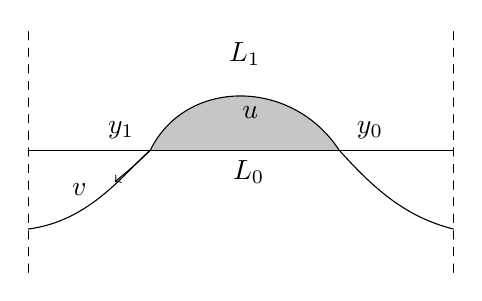
\begin{tikzpicture}[line cap=round,line join=round,scale=1.0]
\draw[dashed] (-2.7,-1.55) -- (-2.7,1.55);
\draw[dashed] (2.7,-1.55) -- (2.7,1.55);
\fill[gray!45] (-1.15,0) .. controls (-0.7,0.92) and (0.65,0.92) .. (1.25,0) -- cycle;
\draw[thin] (-2.7,0) -- (2.7,0);
\draw[thin] (-2.7,-1.0) .. controls (-1.9,-0.9) and (-1.45,-0.25) .. (-1.15,0)
      .. controls (-0.7,0.92) and (0.65,0.92) .. (1.25,0)
      .. controls (1.7,-0.5) and (2.1,-0.85) .. (2.7,-1.0);
\draw[->,thin] (-1.15,0) .. controls (-1.3,-0.15) and (-1.45,-0.28) .. (-1.6,-0.4);
\node at (0.05,1.22) {$L_1$};
\node at (0.12,0.48) {$u$};
\node at (-1.52,0.26) {$y_1$};
\node at (1.64,0.26) {$y_0$};
\node at (0.1,-0.28) {$L_0$};
\node at (-2.05,-0.5) {$v$};
\end{tikzpicture}
\caption{}\label{fig:cylinder-two-gon}
\end{figure}
\end{example}
现在我们要把上述组合构造与真正的\trFukayaCategory{}的\trDirected{}子\trCategory{}
$\scr{F}(\boldsymbol{L}^{\#})^{\to}\subset\scr{F}(M)$ 联系起来。\trObject{}显然相同；%
\trMorphism{}空间也相同，因为 \eqref{eq:combinatorial-index-orientation} 只不过是%
\eqref{eq:pin1-index-orientation} 的重新表述；而且如先前所见，在零维\trModuliSpace{}%
的点 $(r,u)\in\scr{M}^{d+1}(y_0,\ldots,y_d)$ 与\trImmersion{} $(d{+}1)$ 边形%
$\tilde{u}$（在相差\trParametrization{}的意义下）之间存在\trCanonical{}的\trBijective。%
唯一的差别在于：按 \cref{sub:the-fukaya-category} 的一般处方构造\trAinfty{}%
\trStructureMap{} $\mu^d$ 时，所用的是由\trDeterminantLine{}的\trGluing{}论证分析地%
定义的\trIsomorphism{} $c_{r,u}$，见 \eqref{eq:preferred-isomorphism-mu}。更精确地说，%
$\mu^d$ 是把诸贡献 $|(-1)^{\dagger}c_{r,u}|_\KK$ 加起来而得到的，其中 $\dagger$ 如%
\eqref{eq:dagger-sign-exponent} 所设。有鉴于此，把 $\tilde{c}_{\tilde{u}}$ 与%
$(-1)^{\dagger}c_{r,u}$ 之间的符号之差记作 $\gamma^d(\tilde{u})\in\{\pm 1\}$。
我们断言：$\gamma^d(\tilde{u})=\gamma^d(k_d,\ldots,k_1)$ 实际上由所涉交点的绝对%
\trIndex{} $k_j=i(y_j)$ 决定。首先注意，这一符号之差只依赖于我们的几何数据在%
\trImmersion\trPolygon{}附近的局部行为；其次，当我们从 $M$ 过渡到某个\trCovering{}时，%
它保持不变（取诸 $L_{i_k}$ 的\trPreimage，并任取\trPolygon{}的一个\trLift）。利用%
这两点，可以把符号的确定约化到\trPolygon{}是\trEmbedding{}而非\trImmersion{}的情形。%
此时可以沿\trPolygon{}的诸边\trTrivialization{}诸\trLineBundle{} $\beta_{i_k}$，%
这表明 $\gamma^d(\tilde{u})$ 对\trLineBundle{}的一切选取都相同。剩下的局部%
\trTopology{}数据只有绝对\trIndex，这便确立了我们的断言。
\begin{figure}[htbp]
\centering
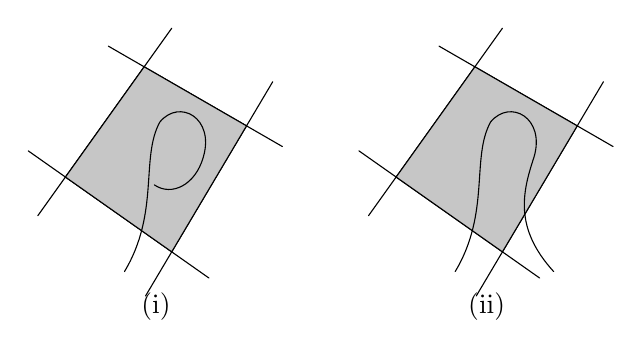
\begin{tikzpicture}[line cap=round,line join=round,scale=1.0]
\begin{scope}[shift={(-1.9,0)}]
\path (0.55,1.5) coordinate (q1) (1.85,0.75) coordinate (q2)
      (0.9,-0.85) coordinate (q3) (-0.45,0.1) coordinate (q4);
\path (q1)--(q2) coordinate[pos=-0.35] (fa) coordinate[pos=1.35] (fb);
\path (q2)--(q3) coordinate[pos=-0.35] (ga) coordinate[pos=1.35] (gb);
\path (q3)--(q4) coordinate[pos=-0.35] (ha) coordinate[pos=1.35] (hb);
\path (q4)--(q1) coordinate[pos=-0.35] (ia) coordinate[pos=1.35] (ib);
\draw[thin] (fa)--(fb) (ga)--(gb) (ha)--(hb) (ia)--(ib);
\fill[gray!45] (q1)--(q2)--(q3)--(q4)--cycle;
\draw[thin] (q1)--(q2)--(q3)--(q4)--cycle;
\draw[thin] (0.3,-1.1) .. controls (0.75,-0.35) and (0.5,0.35) .. (0.75,0.8)
      .. controls (1.0,1.1) and (1.45,0.85) .. (1.3,0.35)
      .. controls (1.2,0.0) and (0.9,-0.15) .. (0.68,0.0);
\node at (0.7,-1.55) {(i)};
\end{scope}
\begin{scope}[shift={(2.3,0)}]
\path (0.55,1.5) coordinate (q1) (1.85,0.75) coordinate (q2)
      (0.9,-0.85) coordinate (q3) (-0.45,0.1) coordinate (q4);
\path (q1)--(q2) coordinate[pos=-0.35] (fa) coordinate[pos=1.35] (fb);
\path (q2)--(q3) coordinate[pos=-0.35] (ga) coordinate[pos=1.35] (gb);
\path (q3)--(q4) coordinate[pos=-0.35] (ha) coordinate[pos=1.35] (hb);
\path (q4)--(q1) coordinate[pos=-0.35] (ia) coordinate[pos=1.35] (ib);
\draw[thin] (fa)--(fb) (ga)--(gb) (ha)--(hb) (ia)--(ib);
\fill[gray!45] (q1)--(q2)--(q3)--(q4)--cycle;
\draw[thin] (q1)--(q2)--(q3)--(q4)--cycle;
\draw[thin] (0.3,-1.1) .. controls (0.75,-0.35) and (0.5,0.35) .. (0.75,0.8)
      .. controls (1.0,1.1) and (1.45,0.85) .. (1.3,0.35)
      .. controls (1.15,-0.1) and (1.05,-0.55) .. (1.55,-1.1);
\node at (0.7,-1.55) {(ii)};
\end{scope}
\end{tikzpicture}
\caption{}\label{fig:sign-decompositions}
\end{figure}
我们还有一条\trApriori{}的信息，即 $\mu^d$ 与 $\tilde{\mu}^d$ 都满足\trAinfty-%
结合性方程。这对诸符号 $\gamma^d$ 施加了相当严格的约束。例如，看一看%
\cref{fig:sign-decompositions}~(i) 所示的那类分解便可看出
$\gamma^d(k_d,\ldots,k_{n+1},k_n+1,\ldots,k_1)\gamma^1(k_n)=\gamma^d(k_d,\ldots,%
k_{n+1}+1,k_n,\ldots,k_1)\gamma^1(k_{n+1})$ 与 $\gamma^d(k_d+1,k_{d-1},\ldots,k_1)%
\gamma^1(k_d)=\gamma^d(k_d,\ldots,k_1)\gamma^1(k_1+\cdots+k_d+2-d)$。经一次初等的%
运算，这就蕴含
\begin{equation*}
\frac{\gamma^d(k_d,\ldots,k_1)}{\gamma^d(0,\ldots,0)}
=\frac{\Gamma(k_1)\Gamma(k_2)\ldots\Gamma(k_d)\Gamma(k_1+\cdots+k_d+2-d)}
       {\Gamma(2-d)},
\end{equation*}
\begingroup\tolerance=9999\emergencystretch=3em\hbadness=10000
其中 $k\ge 0$ 时 $\Gamma(k)=\gamma^1(0)\gamma^1(1)\cdots\gamma^1(k-1)$（而当 $k<0$%
时 $\Gamma(k)=\gamma^1(k)\gamma^1(k+1)\cdots\gamma^1(-1)$）。把一个类似的论证用于%
\cref{fig:sign-decompositions}~(ii)，便表明 $\gamma^d(k_d,\ldots,k_{n+1},\ldots,k_1)%
\gamma^1(k_n)=\gamma^{d-1}(k_d,\ldots,k_n+k_{n+1},\ldots,k_1)\gamma^2(k_{n+1},k_n)$，%
由此得出 $\gamma^d(0,\ldots,0)=\gamma^2(0,0)^{d-1}\Gamma(2-d)$。作为推论，%
$\scr{F}(\boldsymbol{L}^{\#})^{\to}$ 与 $\widetilde{\scr{F}}(\boldsymbol{L}^{\#})^{\to}$%
由一个简单的\trLinear\trIsomorphism{}联系起来，后者把每个\trFloer{}链群 $CF^k$ 乘以%
$\Gamma(k)\gamma^2(0,0)$。由于这对我们的目的已经足够，我们将不再试图显式地确定%
剩下的符号。\par\endgroup
